% !TEX encoding = UTF-8 Unicode

%!TEX TS-program = xelatex
%!TEX encoding = UTF-8 Unicode

\documentclass[oneside,12pt]{book}
\usepackage[left=2cm,top=1cm,right=1cm,nofoot]{geometry}                % See geometry.pdf to learn the layout options. There are lots.
\geometry{a4paper}                   % ... or a4paper or a5paper or ... 
\usepackage{tabularx}

\usepackage{fontspec,xltxtra,xunicode}
\defaultfontfeatures{Mapping=tex-text}
\usepackage[french]{babel}
\usepackage{listings}
\usepackage{graphicx}
\newcommand\don[5]{
\textbf{#1} \\
#2
\begin{itemize}
\item{ \textbf{jet}: #3}
\item{ \textbf{Cout}: #4}
\item{ \textbf{Page}: #5}
\end{itemize}
\vspace{0.5cm}
}


\title{Loup-Garou en terre celte}
\author{Renaud "ObiWan" Guezennec}
\date{}

%\let\origdescription\description
%\renewenvironment{description}{
%  \setlength{\leftmargini}{0em}
%  \origdescription
%  \setlength{\itemindent}{1em}
%}


\begin{document}

\maketitle \clearpage
\tableofcontents \clearpage

\begin{flushleft}
         
\chapter{La meute}
\section{Les crocs de grès }
\begin{description}
\item[Ludovic Clain (Sven)]{ Étudiant ténébreux }
\item[Dermot O'Conneil (Shérif)]{Le jeune flic du coin, alpha de la meute }
\item[Ruth Sulliven(Red Head Redemption)]{Étudiante en biologie }
\item[Christopher Morvant(Obélix)]{ Étudiant, rugbyman }
\item[Claudia Strauss ]{ La violoniste dérangée }
\end{description}



\clearpage
\section{Ithaeur}
\begin{description}
\item[Nom:]{Ludovic Clain}
\item[Origine:]{France}
\item[Auspice:]{Ithaeur}
\item[Tribu:]{Os de l'ombre}
\item[Profession:]{Étudiant}
\item[Nom de guerre:]{Sven}
\item[Age:]{22 ans}
\item[Histoire:]{ 
Tu es un jeune étudiant en langue. Tu as choisi de faire une année erasmus en irlande pour plusieurs raisons: être enfin seul (plus de parents à supporter) et pour t'amuser un peu : glandouille, soirées étudiantes et jeunes étudiantes. Hélas, ta première transformation a changé tes projets. Ta nouvelle condition te fait comprendre pourquoi tu as toujours été mal à l'aise avec les autres (famille et amis). Cela explique aussi pourquoi, tu as une si grande soif de connaissance en occultisme et phénomènes inexplicables.\\
Te voila maintenant Ithaeur (shaman). Tu commences à prendre conscience de l'importance de ton rôle dans la meute. Tu es le membre qui a le plus d'affinités avec le monde des esprits (Hisile). Ton mentor t'a expliqué tout cela à la suite de ton premier changement. Cela commence à se mettre en place dans ta tête.\\

Cela fait un mois que la meute est formée. C'est une jeune meute, elle a  été créé par décision des meutes environnantes afin de les soutenir dans cette zone.\\

Ce soir, tu as convoqué tes frères de meutes car il est temps pour ta meute d'aller chercher un totem (esprit protecteur de meute). Ton mentor te l'as dit. La lune est en croisant, c'est ton auspice. Il est donc plus facile de commencer cette recherche ce soir. Cela prendra du temps, mais tu sais que ta meute en ressortira plus puissante. En effet, un totem est un esprit qui accepte d'aider une meute de loups-garous en échange, le totem demandera certains sacrifices …\\

Tu es conscient de n'être pas le plus apprécier de ta meute. 
Tu débutes dans ton rôle. Tu as encore tant à apprendre alors que les autres jouent avec leurs nouvelles capacités. 
Tu as une responsabilité envers eux. Claudia (la violoniste) et Dermot (le flic) ont conscience de ce nouveau fardeau. Ruth aime te taquiner quand tu échoues, elle reste une personne de confiance. 
Chistopher te semble moins concerné par votre rôle. Tu te méfies de lui. Tu espères qu'il viendra ce soir.\\
}
\end{description}
\clearpage
\textbf{\large Dons} 
\vspace{0.5cm}

\don{Vision de la Mort}{}{}{}{127}
\don{Œil sur la deux monde}{}{Astuce + Occulte + Sagesse}{}{104}
\don{Sentir la corruption}{}{Astuce + Occulte + Pureté}{}{135}

\clearpage
\section{Cahalithe}
\begin{description}
\item[Nom:]{Claudia Strauss}
\item[Origine:]{Allemagne}
\item[Auspice:]{Cahalithe}
\item[Tribu:]{Maitre de fer}
\item[Profession:]{Violoniste et étudiante}
\item[Nom de guerre:]{Melody}
\item[Liste de dons]:
\item[Age:]{22 ans}
\item[Histoire:]{
Jeune prodige de la musique classique, tu es considérée dans le milieu comme la plus grande violoniste d'Europe. La musique est ta passion. Ton éducation a été principalement orienté pour faire de toi une vraie artiste. Tes parents t'ont beaucoup poussé dans cette voie. Tu ne le regrettes pas même si ton enfance est passée trop vite entre les concours de conservatoires, auditions ou les concerts. Il est assez fréquent pour toi de donner des interviews pour des journaux ou magazines spécialisés. Tu es partie d'Allemagne pour effectuer une année Erasmus en Irlande. C'est le moyen pour toi de respirer un an loin des parents et des médias. Grâce à ta musique, tu es riche (tu roules en porsche). Tes parents font parti de la classe moyenne (vers le haute quand même). \\ 
Depuis très jeune, tu fais des rêves étranges:  un monde nocturne, des créatures immatérielles. Parfois, tes rêves renferment quelques  prémonitions. \\ 
Depuis ta première transformation, ces rêves sont de plus en plus fréquents et détaillés. Tu comprends même ce que tu vois: la Pangée, parfois l'hisile. Tu ne comprends pas pourquoi tu les vois. Ces rêves t'ont valu de nombreuses heures chez un psychiatre et des regards étranges dans tes différentes écoles.\\ 

Tu sais vivre avec et cacher ton côté bizarre, tu es un peu dans la lune. Certaines personnes trouvent ça attachant. Tu es une artiste maintenant. Tu as failli perdre la vie lors de la première crise que ta meute a vécu, (il y a 2 semaines).\\ 

Dernièrement, tu as fait un rêve assez étrange. Une femme belle et triste, vêtue  de blanc, à la peau blanche comme la lune.  Dans ton rêve vous vous êtes longuement regardées puis son visage a légèrement évolué pour former le visage d'une vieille femme. Elle cria de façon très aigu. Le cri fut douloureux, tu te réveillas d'un bond, en sueur. 
Tes parents viennent te rendre visite pour les vacances de printemps, (dans deux semaines). Ils seront accompagnés par les journalistes d'un magazine japonais. Ils veulent t'interviewer pour connaître ton sentiment sur les provocations, de la jeune Asaka Sanikashi. 
Ta rivale de toujours, elle est la meilleure violoniste d'Asie. Les média semblent aimer la rivalité qui vous oppose, ils veulent savoir qui est la meilleure du monde. Tu n'y as jamais attaché grande importance. 
La nuit dernière, tu es allé dans un bar avec ton amie (et coloc) « Trish Horgan », après avoir improvisé quelques mélodies celtiques et bu quelques bières, elle a suivi un jeune homme. Tu n'as pas eu de nouvelle depuis. Rien de très inhabituel de sa part mais tu restes vigilante. \\ 

Ce soir, Sven a demandé la réunion de le meute. Tu le trouves assez cool. Il a l'air de prendre son rôle à coeur. Dermot (le flic) est une personne sage et calme, Tu sais qu'il est le meilleur choix d'alpha. Ruth (Red Head redemption) est un peu trop directe et ne prend pas assez de recul par rapport aux événements. Elle reste une personne de confiance. Christopher est un farouche combattant mais il semble peu enclin à changer de vie.\\ 
}
\end{description}
\clearpage
\textbf{\large Dons} 
\vspace{0.5cm}



\don{Nuit Noire}{coupe la lumière }{Astuce + Larcin + Ruse}{1 volonté}{146}
\don{Les bons mots}{Motivez ses amis ou apaise les tensions (bonus + 2 au test sociaux).}{}{}{117}
\don{Connaitre un nom}{Connaitre le vrai nom d'une personne}{Intelligence + investigation + ruse vs résolution + instinct primal}{}{143}

\clearpage
\section{Elodothe}
\begin{description}
\item[Nom:]{Dermot O'Conneil}
\item[Origine:]{Irlande - Dundalk}
\item[Auspice:]{Elodothe}
\item[Tribu:]{Seigneur des tempêtes}
\item[Profession:]{Jeune Flic}
\item[Nom de guerre:]{Leader}
\item[Age:]{21 ans}
\item[Histoire:]{
Tu es issu d'une famille irlandaise assez pauvre. Tes parents ont 4 enfants. Tu es l' aîné. Tes parents ne pouvaient pas te financer des études supérieures. Tu as donc choisi de trouver du travail. Ton envie de faire le bien t'a conduit à t' engager dans la police. 
Tu espères ainsi protéger et servir ta ville et aider tes concitoyens.\\
Tu vis dans un petit appartement au dessus de chez tes parents, dans un quartier populaire de la ville. Depuis que tu es dans la police les gens de ton quartier te regardent avec dégoût. Tu t'en moques, tu es content d'avoir pu sauver cette petite fille de la noyade. Ou bien d'avoir retrouver les vêtements de femme dans le coffre d'un violeur récidiviste. \\
Sven a demandé à la meute de se réunir. Il doit avoir une bonne raison, sûrement en rapport avec le monde des esprits. C'est une tâche bien difficile qui lui tombe dessus. Tu l'aides comme tu peux dans la limite de ta compréhension. Claudia est volontaire pour participer à la vie de la meute. Le côté individualiste de Ruth t'inquiète un peu. Tu as peur qu'elle se retrouve en danger sans frère pour l'aider. Christopher passe un peu pour une brute mais tu sais qu'il vaut mieux que ça. Il a juste beaucoup de mal à accepter sa nouvelle situation. \\

Comme d'habitude, tu as quitté ton travail vers 16 h. Il y a certains événements que tu as noté : \\
-Le conseil économique de l'europe se réunira à Dundalk, la semaine prochaine.  La préparation de ce sommet rend tout le monde nerveux. \\
-Tu n'as pas eu beaucoup de détails mais un beau voilier se serait échoué sur une plage au sud de la ville. La nouvelle est tombée alors que tu avais déjà fini ta journée. Les équipes partaient sur le lieu quand tu es rentré chez toi.\\
-Plusieurs personnes ont rapporté la disparition de jeunes filles majeures (étudiantes pour la plus part). Vous(la police) ne pouvez pas faire grand chose. Elles sont grandes. \\
-Une série de petits cambriolages a été commit dans de luxueuses villas. \\
Il serait peut-être bon qu'une meute de loup-garou inspecte ça de plus près, un de ces quatre.\\
}
\end{description}
\clearpage
\textbf{\large Dons} 
\vspace{0.5cm}

\don{Sentir la malice}{Permet de repérer des êtres corrompu par des sentiments violents : haine, colère, jalousie.}{intelligence + Empathie + Sagesse vs Calme + instinct primal}{1 point d'essence}{135}
\don{Langue déliée}{ manipulation + entregent + Sagesse vs Calme et instinct primal.}{}{1 point d'essence}{110}
\don{Protection contre les prédateurs}{Avertit les autres prédateurs que ce territoire appartient à un prédateur.}{Présence + intimidation + honneur}{1 point d'essence}{139}

\clearpage
\section{Irraka}
\begin{description}
\item[Nom:]{Ruth Sulliven}
\item[Origine:]{Irlande / Sligo}
\item[Auspice:]{Irraka}
\item[Tribu:]{chasseuse des tenebres}
\item[Nom de guerre:]{Red head Redemption}
\item[Profession:]{Etudiante en biologie}
\item[Age:]{22 ans}
\item[Histoire:]{
-Tu es issue d'une famille irlandaise catholique assez aisée. Tes parents sont propriétaires d'un haras. Ils vendent des chevaux très réputés pour le saut d'obstacles. Ils vivent dans la région de Sligo (côte Ouest au nord de l'Irlande). Tu as vécu dans une famille très “irlandaise”.(Ton père parle le gaélique...)   Depuis toute jeune, tu aimes faire des promenades dans le domaine de tes parents. C'était vital pour toi. Tu accompagnais souvent ton père à la chasse. L'idée de poursuivre une proie est plaisante (la tuer moins), c'est un défi que tu aimes relever. Tu as compris que ton tempérament était provoqué par ta condition de loup-garou. Tu es contente d'avoir pu quitter ta famille pour vivre seule. Tu es à Dundalk pour tes études de biologie. C'est ici que tu as vécu ton premier changement.\\
Tu as compris beaucoup de chose sur toi-même depuis ton premier changement. L'envie de chasser est toujours là, 10 fois plus forte qu'avant. \\

Sven (le français ténébreux) souhaite réunir la meute. Tu sens que la soirée va être drôle. Sven est le genre de personne à crier au loup pour rien. C'est jamais dangereux, ça te fait rire même. Qu'est-ce qu'il vous réserve cette fois ? \\
Dermot a confirmé que la réunion était importante. Dermot est un mec intelligent, il a probablement ses raisons pour confirmer le rendez-vous. Claudia est toujours partante pour tout. Elle est un peu trop dans son monde pour être utile, dans les moments dangereux. Elle a été gravement blessé pendant la rencontre avec la meute des « Pierres Blanches». Christopher est une personne avec qui tu t'entends bien. Vous êtes des personnes d'actions. Il ne semble cependant pas très motivé par cette vie. \\
Enfin dans tous les cas, cette réunion tombe bien. Tu as remarqué des choses étranges, lors de ta ronde la nuit dernière. \\
Une  sorte de secte se réunit sur votre territoire à l'extrémité Nord-est. Tu aimerais bien leur faire comprendre d'aller faire « mumuse » ailleurs. 
Leurs présences troublent les esprits et salissent votre territoire. Ils accomplissent des sortes des rituels païens.  
Tu n'as pas eu le temps de les observer très longtemps. 
Le lieu de rendez vous est une église (Saint-James) en ruine dans un quartier en ruine de la ville. C'est probablement des hippies qui abusent de la « verveine de hollande ».
}
\end{description}
\clearpage
\textbf{\large Dons} 
\vspace{0.5cm}

\don{S'esquiver}{Ce don te permet de te détacher de tes liens. C'est le degré zero de la quête de liberté. Que ce soit une camisole, des menottes ou bien des chaines, tu t'en libères sans les endommagées.}{}{[1 point de volonté]}{132}
\don{Poudre aux yeux}{Les gens ne se souviennent pas de ton passages. }{ manipulation + subterfuge + ruse vs calme + instinct primal}{}{110}
\don{Langue animale}{Parler/écouter avec/un animal. }{Manipulation + Persuation + Honneur}{1 Point d'Essence}{113}


\clearpage
\section{Rahu}
\begin{description}
\item[Nom:]{Christopher Morvant}
\item[Origine:]{France}
\item[Auspice:]{Rahu}
\item[Tribu:]{Griffe de sang}
\item[Nom de guerre:]{Obélix}
\item[Profession:]{Étudiant , rugbyman}
\item[Age:]{20 ans}
\item[Histoire:]{ 
Tu es un étudiant français venu en Irlande pour une année spéciale de perfectionnement de rugby.\\
L'année prochaine, tu devais passer professionnel. Ta première transformation a changé un peu la donne. Tout au long de ton enfance, tu as été colérique et violent, tu comprends maintenant pourquoi. C'est la bête en toi qui à soif de violence. Le sport t'a aidé à calmer ses envies et maintenant que tu es un loup garou, tu fais extremement attention. Tu as vu que se laisser emporter par sa rage pouvait être dangereux pour toi et pour tes frères de meute.\\
Tu apprends à te calmer et être plus utile à la meute. Cependant, tu regrettes tellement ton ignorance sur le monde des esprits, cela t'intrigue beaucoup. Tu as l'impression que tout le monde te prends pour plus idiot que tu n'es. Tu es le plus jeune loup-garou de la meute.\\
Tu sais que Dermot (le flic) calme un peu souvent tes initiatives. 
Claudia t'ignore plus qu'autre chose. Ruth est sympa, elle t'aide. 
Vous êtes un peu semblable : des personnes qui aiment l'action. 
Sven est probablement le plus pince sans rire avec toi. 
Il te taquine, c'est qui a trouvé ton nom de guerre. 
C'est surement un moyen de soulager ses propres angoisses. Vous êtres français tous les deux. 
Cela fait deux jours que ta copine ne répond pas à tes coups de fil. Ta relation avec elle bat de l'aile. Elle avait rendez-vous avec des copines dans un bar avant-hier soir (Déborah). Depuis plus de nouvelles, elle doit faire ça pour t'énerver et te rendre jaloux et cela marche. 
}
\end{description}
\clearpage
\textbf{\large Dons} 
\vspace{0.5cm}

\don{Changement partiel}{Tu peux changer une partie de ton corps dans la forme loup-garou que tu veux. Tu peux par exemple rester humain et changer uniquement ton nez afin d'améliorer ton sens olfactif pour chasser un adversaire. }{vigueur + survie + instinct primal}{1 point de volonté}{121}
\don{Volonté de Luna}{Le sujet obéit à un ordre de quelques mots. }{présence + intimidation + Gloire vs Calme + instinct primal}{}{107}
\don{Clarté}{+5 au jet d'init. Peut aider pour attaquer le premier.}{}{1 point d'essence}{138}

\chapter{L'histoire commence}
\section{Informations aux PJ}
\section{La meute des PJs : Les crocs de grès }
\begin{description}
\item[Ludovic Clain (Sven)]{ A demander le rassemblement de la meute pour aller chercher un totem (c'est la lune en croissant) }
\item[Dermot O'Conneil (Leader)]{Les divers petits vols et effractions dans des villa au sud de la ville, préparatifs du sommet irlande nord-sud, bateau échoué au sud de la ville. }
\item[Ruth Sulliven(Red Head Redemption)]{ Rituel bizarre avec des animaux morts au sud ouest de la ville (ce sont les 7 crinières qui font des tests) }
\item[Christopher Morvant(Obélix)]{ Copine disparue }
\item[Claudia Strauss (Melody)]{ amie disparue et parents qui vont bientot venir }
\end{description}


\section{Scène 1 : La poursuite d'un totem}
C'est le croissant de lune, la date idéale pour notre jeune meute de rechercher un totem. Cela ne se fera peut-être pas en une soirée mais il faut commencer. 
Ainsi toute la meute est regroupée au locus (un dolmen) à l'extérieur de la ville. \\
Vous pouvez ici lancer la chasse, faire une course poursuite: Astuce + survie (irraka), vigueur + sport pour la course.
Pendant la course, il vont croiser Fintan.

\section{Scène 2 : Fintan}
Fintan est un esprit très ancien qui va demander à la meute de lui ramener le scatham glas. Un fétiche puissant qui lui appartient.\\
En échange, il proposera à la meute de gagner un don ou de les aider à trouver un totem… Fintann ne sait pas à quoi ressemble le fétiche mais il sait qu'il est sur le territoire de la meute. Il imposera une limite de temps (en gros 6 à 12h). S'il estime qu'ils ont pris trop de temps pour le trouver. Il ne sera pas généreux.
C'est un esprit très puissant.
Physiquement, il est mi-homme; mi-poisson (décrire en détails des portions de bras avec des écailles, des bouts de nageoires..). Il sent fort le poisson. Malgrès cela, les personnages féminin pourrait resentir un certain désir, rien d'incontrôlable mais tout de même.


\section{Scène 2bis : La banshee}
Alors que toute la meute parle à Fintan, Claudia la Cahalithe du groupe, va entendre une voix l'appeler. La voix dit «Elle va revenir, l'ivresse est là»,«Elle règnera encore une fois».\\ Claudia pourra voir une jeune femme toute blanche, vétue de draps blancs, le visage dissimulé, elle livrera le message et hurlera d'une voix stridente. La femme se transformera en 3 oies, et ils prendront leurs envols.
Claudia peut faire un test de resolution + calme pour ne pas tomber dans les pommes quelques instants. Les cri de douleur de Claudia alerteront ses camarades de meute.

\section{Scène 3: le scatham glas}
Il est possible d'apprendre des infos sur cet objet sur internet.\\
Une recherche renverra comme réponse :
\begin{itemize}
\item Site web de Isabell Blunt, photographe canadienne ayant fait une série de photo "Scatham", qui montre des jeux de miroir.
\item Page d'homonymie de Wikipédia : avec une page sur Isabell Blunt, une page sur les bijoux fantaisie Irlandais. 
\item Le site myspace d'un groupe de folk métal de Boston
\end{itemize}
La seule page vraiment utile, c'est les bijoux.
Sur la page wiki, il y a des photos de plusieurs broches, trisquel, croix diverse. Ces bijoux sont principalement tous fabriqués par la société : Irish Jewelry
La plus part des design sont inspirés d'objets retrouvés dans des fouilles ou sur des rochets.\\
L'article montre en exemple le fameux : Scatham glas, retrouvé, il y a 50 ans sur une plage du comté du Kerry.
Personne ne sait d'ou vient cette pièce, il est également impossible de la dater.\\
Le miroir vert en gaélique: Sorte de trisquel vert en pierre dans une enveloppe de verre.\\
L'actuel possesseur du scatham glas est un certain : Duncan O'Reilly\\

En général, je ne fais par trop perdre de temps à mes joueurs pour savoir qui possède maintenant le scatham glas. Vous pouvez livrer les informations plus difficilement. \\
Je n'ai jamais été très satisfait de cette scène là. Si vous avez d'autres idées pour donner ses infos, n'hésitez pas. \\

\section{Scène 4 : famille O'Reilly}
\begin{description}
\item[Père] : Duncan (Grand scientifique en biologie et neurologie)
\item[Mère] : Mary
\item[Fille ainée] : Jenny
\item[Fille]: Lisy
\item[le bateau] : Jenny (Comme l'ainée)
\end{description}
La découverte du nom va amener les joueurs à faire une recherche sur les O'Reilly.
Le père est un grand scientifique en neurologie et en pharmacie. Il est devenu très riche grace à quelques médicament très efficaces.
Tellement riche, qu'il ne travaille plus, sa compagnie lui appartient, il a des ingénieurs qui bossent pour lui maintenant. 
Il en profite pour faire le tour du monde en voilier avec sa famille.
Jenny tient un blog/carnet de voyage. Le dernier poste date d'une grosse semaine. Ils étaient au large de l'irlande.
Une carte signale leur route, ils devraient normalement être à Dublin pour un festival de grand voilier ĥistorique. 

Normalement, il faut donner suffisament de détail pour que le flic fasse le rapprochement avec le bateau échoué.
Il faudra que Dermot appelle ses amis en poste pour avoir des infos: lieux précis …
Il apprendra que l'armée britanique s'occupe du truc, la police d'irlande ne fait rien. Cela vient de très haut.

\subsection{Information sur Dundalk}
Dundalk est une ville de 50 000 habitants (assez grosse ville pour l'Irlande). 
Elle est situé à 80km de Dublin et 80km de Belfast.
La ville est en République d'Irlande, mais seulement à 4 km de la frontière avec l'Irlande du nord. 
La ville est connu pour son institue de technologie: DKIT ( http://ww2.dkit.ie/ ) 
Il reçoit beaucoup d'étudiant étrangers. Les étudiants vivent sur le campus dans un batiment apart.
Appartement pour 5 personnes, mixtes. Claudia, Christopher, Ruth et Ludovic vivent dans ce batiment.
Dermot lui vit au dessus de chez ses parents en ville.

\section{Scène 5 : Le bateau}
La zone du bateau est très inaccessible. Il faut traversé une forêt pour tomber sur une grande plage.
Le bateau est gardé par 2 soldats anglais. Il y a des grues et autres gros engins. Ils y a des projecteurs un peu par tout. 
De la lisière de la foret au bateau, il y a 100m à decouvert et plein de lumière. Les soldats ont des armes lourdes mais ne semble pas très vifs.
C'est le moment parfait pour Claudia d'utiliser son don «Nuit noire».
Après cela, entrer dans le bateau est très facile. 

Le navire est constitué de deux escaliers qui menent au milieu du bateau. D'un coté le salon, de l'autre les chambres et le poste de pilotage.

Voir schéma:
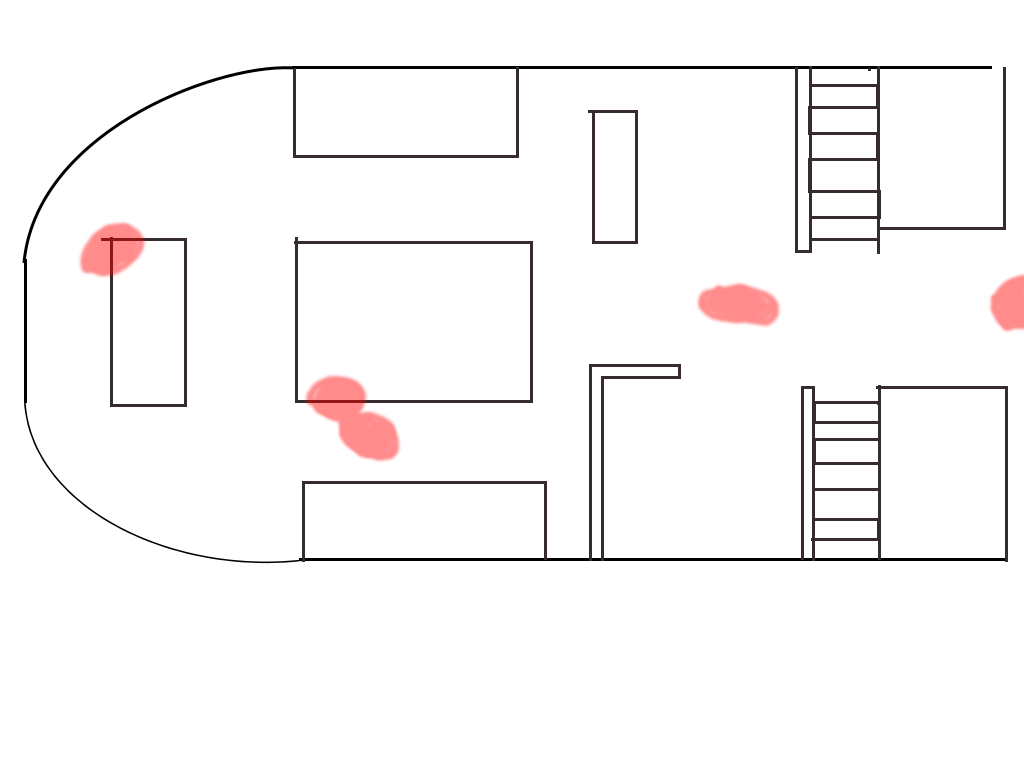
\includegraphics[scale=0.5]{bateau.png} \\
Les traces rouges sont des marques de sang. Le bateau a été fouillé et les corps ne sont plus là. 
De gauche à droite: Jenny, la mère, un ravisseur, le père et le dernier ravisseur.
La température de la pièce est froide, surnaturellement froide même. Le fantôme de la mère est là. Seul l'utilisation de vision de la mort permet de le voir et de communiquer avec le fantôme.
Le fantôme est comme un disque en boucle:  «Chérie où es-tu? C'est maman»

Ce que les joueurs peuvent comprendre:
Il n'est sencé y avoir que 4 personnes à bord mais il y a 5 trace de sang. Les morts semblent violentes, beaucoup de sang. 
Dans les chambres, il manque beaucoup de vetement surtout pour Lizy. Dès qu'ils comprennent qu'une personne a peut-être survécu, il faut lancer l'attaque. 

A ce moment là, un coup feu éclate (un jeu de astuce + arme à feu permet de remarquer qu'il y a eu deux coups en même temps. Des commando entre dans le bateau bombarde de grenade lacrymo, flash et tout et Tazze le PJ. 
Ils sont fait prisonier. 


\section{Scène 6 : Les mercenaires}
Les joueurs sont transportés, mains dans le dos, dans une vieille fabrique de bière. Ils sont tous jeter dans des cuves d'acier. Les commandos repart illico (ils vont attaquer l'hopital pour rechercher les cadavres et espérer trouver ce qu'ils cherchent). Seul, 2 personnes restent pour interroger les joueurs. Ils choissiront Red Head Redemption comme première victime. \\
Les mercenaires vont essayer de savoir "où est la carte mémoire?". \\
Utilisation du don, Petit combat, elle gagne assez facilement. Il restait seulement un jeune et un vieux mercenaires. Le vieux pose les questions et le jeune tape. En général, la simple vue d'un uratha en forme guerrière suffit à rendre le jeune complètement fou. Le vieux est plus corriace. \\

Ce lieu est le QG des mercenaires, ils ont 2 raisons d'être ici. Le premier contract est de retrouver la puce mémoire qui est attaché au scatham glas. 
La deuxième raison c'est de kidnapper des jeunes filles pour une secte. 

Dans l'usine, il est possible de trouver, un tas de téléphone portable très "girly" (rose avec des coeurs..).  La pièce est pleine d'électronique, des écrans branchés sur le réseau de vidéo surveillance de la ville..
Les Pj peuvent voir l'attaque du commissariat sur les écrans. 

A ce moment, l'un des téléphones va sonner, de l'autre côté du fil: Henry Bedford - le patron de la pharmacorp. Entreprise concurrente de celle de Duncan O'Reilly.
Cet homme est possédé par un esprit d'"ivresse du pouvoir" (soit la déesse Medb chez les celtes). 
C'est lui qui paye les mercenaires pour trouver la puce. Qu'importe la personne si on lui rapporte la puce , il payera beaucoup (Inspiration pour le personnage, Zorg dans le 5ème élément). 
Les personnages peuvent lui faire croire qu'ils ont la puce, ou juste lui raccrocher au nez. La prophécie de la banshee parle de lui. C'est son retour (ou le retour de Medb qu'elle a prédit). La puce informatique contient un virus très puissante créer par Duncan quand il était étudiant, c'est un pari qu'il avait fait avec H.Bedford pendant l'université. H.Bedfort veut lacher son virus et celui de duncan pour voir lequel est le plus meutrier.   

H.bedford est à la tête d'une entreprise familliale grosse entreprise qui se fait rattraper petit à petit par le petit poucet qu'est l'entreprise d'O'Reilly.

Si les Pj interrogent les deux mercenaires. Ils ne seront que peu de chose sur le groupe qui se charge des filles. Juste que c'est un contrat et qu'ils sont parti vers le sud (vers Drogeda ou Dublin).

Dans le local des mercenaires se trouve un ordinateur avec un autocollant "Hawkson industries", il est chargé de décoder la mémory stick et envoyer le contenu directement sur un site sécurisé. 



\section{Medb : la bad girl: Rebecca Hawkson}
Une voie féminine les contactera dans le hall des mercenaires, ils seront insulté pour leur incompétence. 
C'est la présidente de Medb corp, une entreprise pharmacologie, laboratoire etc.. qui est commandé par une certaine Rebecca Hawkson. Il y a deux mois son entreprise à changer de nom pour devenir Medb corp (avant c'était Hawkson Industries). Elle a été la petite amie de Duncan O'Reilly à la fac. 
Sa soif de pouvoir et sa jalousie on rendu le terrain propice pour une possession par un esprit.    

\section{Scène 7 : Lizy}
Lizy est la cadette (8 ans) de la famille O'Reilly, elle se trouvait à bord du navire. Elle porte le scatham glas (ainsi que la carte mémoire). Elle est possédé par un 
esprit de la gourmandise. 
Dans le bateau avec sa famille, 2 commando l'ont pris de force. Après plusieurs heures de prise d'otages, interrogatoire, hurlement, le père s'est interposé, il a été tué ainsi que sa femme et sa fille. Lizy s'était cachée dans sa chambre. Seul un esprit de la gourmandise la aider (elle est très gourmande). Elle a ainsi tuer  les deux agresseurs (et les a manger en partie). 
Puis le bateau à dériver pendant quelques jours pour s'arriver sur la côte. Pendant ces quelques jours, Lizy s'est caché dans la cale du navire, pour ne pas voir le massacre. Avant de sortir, pousser par la faim, elle a pris le Scatham glas (son père lui avait dit qu'il était important pour la famille). Elle est allé se réfugier dans des maisons de vacances à 1-2 km du bateau. Elle a trouvé une cabane où elle s'est réfugiée.
Elle a volé quelques bonbons dans les maisons voisines. 

Les joueurs devront chercher l'odeur de la petite fille dans le bateau, puis la pister maintenant qu'ils savent quoi chercher. L'odeur est partout dans la forêt.
La fille pue, elle est couverte de sang, vetement sales. Ils la retrouvent dans la cabane en haut d'un arbre. C'est le moment de faire du social (Claudia). 
La fille aura plus facilement confiance avec Claudia (enfin c'est un conseil pour que chaque joueur est un quart d'heure de gloire). 
Les PJ peuvent faire tous les dons qu'ils veulent tant qu'elle porte le scatham glas, on ne voit rien. 


\section{Scène 8 : Rendre le fétiche a Fintan}
Pour rendre le fétiche, il faut aller dans l'hisil. La carte mémoire est collé et camouflé dans le fétiche, mais elle ne peut pas aller dans l'hisil. Il faut faire attention à
qui tient le fétiche et l'ordre de passage vers l'hisil.  
Dans l'hisil, le fétiche ressemble à une flemme verte. 
Quand Fintan reçoit le fétiche, la flamme verte reste dans sa main alors que l'objet passe au travers. L'aspect de Fintan, se transforme, il devient un homme spendide.
Il remercie les PJ par un don, Fintan étant un esprit de la survie, il leur donnera le don de connaissance de meute. 

\section{Scène 8bis : Contenu de la carte mémoire (facultatif) } 
Les pj peuvent vouloir étudier le contenu de la carte. Rien ne semble lisible sur un pc commun. Les PJ doivent rechercher un expert. Ça tombe bien, 
il y a un batiment rempli d'étudiants dont certains en informatique.
Il demandera surement un rdv avec une des deux filles de la meute en échange.
Cela lui prendre du temps (24h) pour avoir les premières informations. 
C'est dans la globalité des documents professionels, des compositions chimiques de médicaments, un virus. 

\section{Scène 9 : Les pouvoirs du scatham Glas}
Le fétiche empèche toute manifestation d'un pouvoir spirituel. Les dons (qui font des cadeaux des esprits sont paralysés).
Si un uratha porte le scatham glas, il ne peut pas se transformer (il reste en humain). Il peut lui se croire en Urhane ou Urshul etc. C'est assez amusant de jouer ce truc. 
Si Lizy  est observée sans le scatham glas (attention si le loup garou qui utilise un don porte le fétiche il ne vera rien non plus), elle laisse appercevoir des dents monstrueuses, des lambeaux de chair entre les dents, une musculature assez importante. Alors que sans le don, elle ressemble a une fille de 8 ans un peu rondouiette.   
Insister sur le faite qu'elle veut manger. Elle ne voudra pas se séparer du fétiche volontairement. Parcontre lui voler pendant son sommeil ou de force n'est pas bien dur. Si elle porte le scatham glas est qu'elle est proche du locus de la meute. Elle ira donné le fétiche à Fintan.
Elle peut essayer de mordre un pj. Grosso modo, si les PJ la laisse seule sans le fétiche pour contrer l'esprit de la gourmandise. Elle fera un carnage.


\section{Scene 10: Jessica Hawkson arrive}
Comme prévu, elle vient accomplir son expérience, elle a grandement besoin de récupérer la puce. Un laboratoire clandestin a été installé dans les sous-sols de l'église ou dans le quartier. Elle apprendra par les mercenaires qu'un autre groupe de gens est sur les traces de la puce. 


\section{Scène 10 : Le sacrifice des 7 crinières}
Les 7 crinières sont dans la mythologie celte, les garde de la déesse de la Guerre Morrigan.
Il travaillent sous les autres d'une femme, très jolie rousse 35 ans(Medb) . Les victimes sont plaquées ventre contre une estrade et sont violés par les 7 ritualistes. 
Pendant les viols, elle se masturbe. Dès que les Pj se montrent, elle s'enfuira en lachant un poison, Ils vont tousser. C'est la chef de la Medb corp, elle est possédée par un esprit du pouvoir, elle se prend donc pour medb. 
 
\begin{itemize}
\item Fedlimid became Maine Athramail ("like his father")
\item Cairbre became Maine Máthramail ("like his mother")
\item Eochaid became Maine Andoe ("the swift")
\item Fergus became Maine Taí ("the silent")
\item Cet became Maine Mórgor ("of great duty")
\item Sin became Maine Mílscothach ("honey-speech")
\item Dáire became Maine Móepirt ("beyond description")
\end{itemize}


Dans le scénario, ce sont 7 aristocrates qui font une sectes d'adorateur de Morrigan. Ils vont sacrifier les jeunes filles dans l'église Saint-James.
Le rituel peut marcher ou non à vous de voir. S'il marche Morrigan défonsera tous le monde de la secte et "droguera" les PJ. Puis repassera dans un locus. 
Si morrigan se montre, toutes les actions des PJ sont limités à un dés (c'était un pouvoir de Morrigan: aider les guerrières, ou les affaiblir)
Dans tous les cas, dans les victimes il y a la petite amie de Christopher et l'amie de Claudia (rage mortelle ?). 
 




\section{Que fait l'armée ?}
L'armée anglaise a été informé par les USA de la présence de cette puce


\section{Inspiration}
Je vous conseille fortement de lire des documents sur "La razzia des vaches de Cooley" et medb : http://fr.wikipedia.org/wiki/Medb.
A la place des taureaux, se sont des virus. 

Fintan est l'un des premiers hommes a être venu en irlande,  http://fr.wikipedia.org/wiki/Fintani\_%28mythologie_celtique%29
Il s'est échapé en sautant dans la mer en se changeant en sommon.

Les septs crinières sont le nom de soldat de Morrigan. 

\end{flushleft}
\end{document}
